\documentclass[conference]{IEEEtran}
\IEEEoverridecommandlockouts
\usepackage{cite}
\usepackage{amsmath,amssymb,amsfonts}
\usepackage{algorithmic}
\usepackage{graphicx}
\usepackage{textcomp}
\usepackage{xcolor}
\usepackage{rotating}
\usepackage[nottoc]{tocbibind}
\usepackage{hyperref}
\def\BibTeX{{\rm B\kern-.05em{\sc i\kern-.025em b}\kern-.08em
    T\kern-.1667em\lower.7ex\hbox{E}\kern-.125emX}}


\begin{document}

\title{Image Guided Robotic Needle Placement}

\author{\IEEEauthorblockN{Aishwarya Krishnamurthy, Chinmay Sujir, Konika Khatri,\\ Mansi Dayama, Orhun Cenk Taskin, Sriramkumar Sarida }
\IEEEauthorblockA{\textit{Institute of Medical Technology at Hamburg University of Technology,} \\
\textit{Am Schwarzenberg-Campus 3, 21073 Hamburg, Germany}\\
Hamburg, Germany \\
aishwarya.krishnamurthy@tuhh.de, chinmay.sujir@tuhh.de, konika.khatri@tuhh.de,\\ mansi.dayama@tuhh.de, orhun.taskin@tuhh.de, sriramkumar.sarida@tuhh.de}}

\maketitle

\begin{abstract}
    Needle placement into the patients body is a necessary process employed in surgical applications.
Using modern techniques of robotics and image processing this process can be improved in terms of precision and safety.
This document outlines the implementation of the needle placement by a robot manipulator as a part of course work in Robotics and Navigation in Medicine at Hamburg University of Technology (TUHH).
\end{abstract}

%\begin{IEEEkeywords}
%component, formatting, style, styling, insert
%\end{IEEEkeywords}

\section{Introduction}
In medical procedures(e.g.\ biopsies, drug insertions) medical needles are used as insertion tools into the patients body.
Considering the delicate structure of the surrounding tissue and the following healing process it is imperative to improve this process for increased safety and precision.
Using robots to guide the needle to the desired position is a viable alternative to the manual insertion by a surgeon, and holds possibilities for such improvements. These advancements can be accomplished with modern 3D imaging techniques and trajectory planning.

In this project aim is to develop robotic needle placement system guided by image processing techniques.
Project framework is to use Robotic Operaing System (ROS) in conjunction with the depth camera (Kinect Azure by Microsoft) mounted on the surgical robot arm (Panda by Franka Emika).
In this manner, depth camera will give the necessary visual information to drive the needle to the target position while the kinematics package driving robot to the required positions.

In this document we present a report of the results of this project as a part of the aforementioned course.
The paper is organized in two major sections, namely Kinematics and Vision explaining the implementation in detail, followed by Discussion and Conclusions, among which the former includes the Contributions part where participants explain their share of the workload.

\section{Kinematics}
Kinematics, often regarded as 'geometry of motion' describes motion of points (or bodies) without considering the effect of forces \cite{wikikine}. Kinematics can be separated into four steps, which are namely forward and inverse kinematics, path and trajectory planning. In this section we will first introduce the theoretical background of the aforementioned four steps then outline the implementation that arose from this theory.
\subsection{Theory}


\subsubsection{Forward Kinematics}
Forward kinematics is the problem of determination of the position and orientation of the end effector given the values for the joint variables. One common way to approach this problem is via utilizing Denavit and Hartenberg (D-H).
In D-H convention each joint is attached with one coordination frame and transformation between these frames are
expressed in four parameters \cite{wikidh}
\begin{itemize}
    \item $d$: offset along previous $z$ to the common normal
    \item $\theta$: angle about previous $z$, from old $x$ to new $x$
    \item $a$: length of the common normal. Assuming a revolute joint, this is the radius about previous $z$
    \item $\alpha$: angle about common normal, from old $z$ axis to new $z$ axis
\end{itemize}
Using the modified version of the DH-parameters results in transformation matrix between axes $n-1$ and $n$ as follows

\begin{equation}
    ^{n - 1}T_n=
    \left[\begin{smallmatrix}
              \cos\theta_n & -\sin\theta_n  & 0 & a_{n-1} \\
              \sin\theta_n \cos\alpha_{n-1} & \cos\theta_n \cos\alpha_{n-1} & -\sin\alpha_{n-1}& -d_n
              \sin\alpha_{n-1} \\
              \sin\theta_n\sin\alpha_{n-1} & \cos\theta_n \sin\alpha_{n-1} & \cos\alpha_{n-1} & d_n
              \cos\alpha_{n-1} \\
              0 & 0 & 0 & 1
    \end{smallmatrix} \right]
\end{equation}
So given all DH-parameters one can find all coordinate frames defined on the robot. These parameters can be presented
on a table, named appropriately as DH-Table, which is commonly provided by the manufacturer. In this case the table
provided by Franka documentary is tabulated in Table \ref{dhtable}. More info can be found on website of Franka Control Interface \cite{frankaweb}.

\begin{table}[ht]
    \caption{DH-parameters}
    \label{dhtable}
    \begin{center}
        \begin{tabular}{|c|c|c|c|c|}
            \hline
            \textbf{\textit{Joint}} & \textbf{\textit{a (m)}} & \textbf{\textit{d (m)}} & \textbf{\textit{ $\alpha$
                (rad)}}& \textbf{\textit{ $\theta$ (rad)}}\\
            \hline
            Joint1 & 0 & 0.333 & 0
            & $\theta_{1}$ \\
            \hline
            Joint2 & 0 & 0 & -$\pi$/2
            & $\theta_{2}$ \\
            \hline
            Joint3 & 0 & 0.316 & $\pi$/2
            & $\theta_{3}$ \\
            \hline
            Joint4 & 0.0825 & 0 & $\pi$/2
            & $\theta_{4}$ \\
            \hline
            Joint5 & -0.0825 & 0.384 & -$\pi$/2
            & $\theta_{5}$ \\
            \hline
            Joint6 & 0 & 0 & $\pi$/2
            & $\theta_{6}$ \\
            \hline
            Joint7 & 0.088 & 0 & $\pi$/2
            & $\theta_{7}$ \\
            \hline
            Flange & 0 & 0.107 & 0 & 0 \\
            \hline
        \end{tabular}
        \label{tab2}
    \end{center}
\end{table}

Utilizing this table one can calculate the end effector pose by multiplying each transformation. This equation as commonly called kinematic chain can be found below in Equation \ref{chain_eq}.

\begin{equation}
    \label{chain_eq}
    T_7^0 = T_1^0 T_2^1 T_3^2 T_4^3 T_5^4 T_6^5 T_7^6
\end{equation}

Figure \ref{robot_img} depicts the provided frames on the robot image.


\begin{figure}[ht]
    \centering
    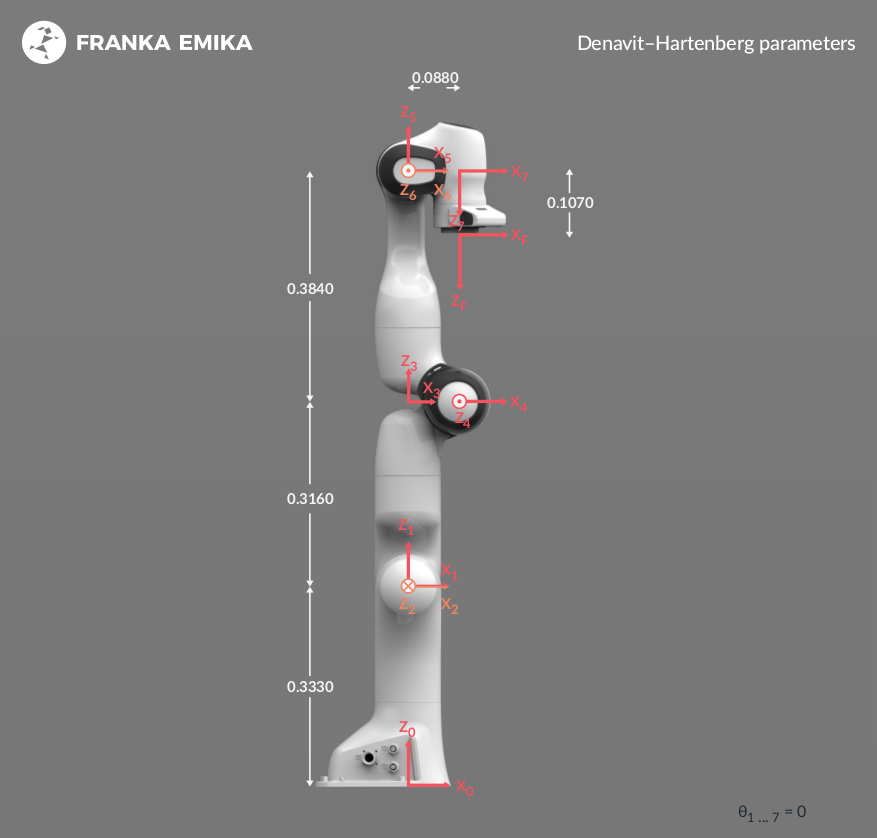
\includegraphics[width=0.45\textwidth]{images/dh-diagram.png}
    \caption{Coordinate frames on the robot}
    \label{robot_img}
\end{figure}

\subsubsection{Inverse Kinematics}
As forward kinematics determine the position and orientation of the end effector from joint variables, inverse kinematics determines the latter given the former. More generally, given a homogeneous transformation
$$
H = 
\begin{bmatrix}
R & p \\
0 & 1
\end{bmatrix}
$$
find joint variables
$$
T_n^0(q_1,...,q_n) = H
$$
Although there are closed form solutions to the system of equations, as geometry of robot gets more complex they become hard to solve analytically. In this study we used a common approach to approximate the solution of systems, namely least squares. The least-squares method finds the optimal parameter values by  minimizing the sum of squared residuals

$$S=\sum_{i=1}^{n}r_i^2.$$
\subsubsection{Path Planning}
Path planning aims to find a continuous map $g$ from start point, $g(0)$ to goal point $g(1)$ in configuration space, taking into account where the known world $W$ is occupied by obstacles or with the robot itself. With the inverse kinematics we can map these points to their corresponding configurations, namely $q_s$ and $q_g$.

In this study we don't consider obstacles, so motion planning simplifies to trajectory generation, which is enough to 'move' the robot from its former pose into the goal position with a simple check on joint limits.
\subsubsection{Trajectory Generation}
 A trajectory is a function of time $q(t)$ such that $q(t_0)=q_s$ and $q(t_f)=q_g$ (see Trajectory Planning section in \cite{spong}). Trajectory planning expands the path into a 'step-by-step plan' with the introduction of time as a variable, which than could be fed to the controller. Here 'step-by-step' posits the implicit dependency on control frequency, which in case of Panda robot is 1000Hz.
 
 Polynomials of degree n, is a common selection for parametrization of trajectories, where n is dependent on the number of constraints \cite{spong}.Having continuous position, velocity and acceleration (thus no impulsive jerk) for both initial and final configurations lays 6 constraints, so a fifth order polynomial
$$ q(t) = a_0 + a_1t + a_2t^2 + a_3t^3 + a_4t^4 + a_5t^5 $$
would suffice. Taking its derivatives one could reach at:
$$ v(t) = \Dot{q}(t) = a_1 +2 a_2t +3 a_3t^2 +4 a_4t^3 +5 a_5t^4 $$
$$ \alpha(t) = \Ddot{q}(t) = 2 a_2 + 6 a_3t + 12 a_4t^2 + 20 a_5t^3 $$
Plugging $t_0$ and $t_f$ in to above equations and then arranging them in matrix form:
$$\begin{bmatrix}
1 & t_0 & t_0^2 & t_0^3 & t_0^4 & t_0^5 \\
0 & 1 & 2t_0 & 3t_0^2 & 4t_0^3 & 5t_0^4\\
0 & 0 & 2 & 6t_0 & 12t_0^2 & 20t_0^3\\
1 & t_f & t_f^2 & t_f^3 & t_f^4 & t_f^5\\
0 & 1 & 2t_f & 3t_f^2 & 4t_f^3 & 5t_f^4\\
0 & 0 & 2 & 6t_f & 12t_f^2 & 20t_f^3\\ 
\end{bmatrix}
\begin{bmatrix}a_0\\a_1\\a_2\\a_3\\a_4\\a_5\\\end{bmatrix}
=
\begin{bmatrix}q_0\\v_0\\\alpha_0\\q_f\\v_f\\\alpha_f\end{bmatrix}$$
Solving this linear system of equations would result in coefficients $a_i$ that can be used to parametrize the trajectory in the appropriate profiles. These profiles can be seen on Figure \ref{quintics}

 \begin{figure}[ht]
  \centering
  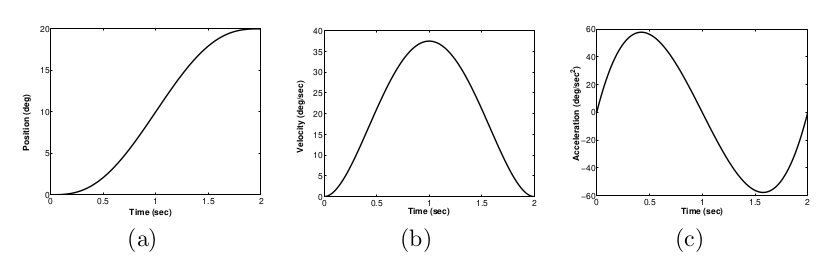
\includegraphics[width=0.45\textwidth]{images/quintics.png}
  \caption{(a) Quintic Polynomial Trajectory. (b) Velocity Profile  (c) Acceleration Profile (figure obtained from \cite{spong}])}
  \label{quintics}
 \end{figure}


% Tell how we used changed frankaros
\subsection{Implementation}
When divided into two main packages the runtime process simplifies to following steps:
\begin{itemize}
    \item Kinematics: Scans the target provides requested image and pose pairs to the vision package
    \item Vision: Processes aforementioned inputs to provide 3-float vector corresponding the position of the target point, accompanied by information on the possible approach orientation for insertion.
    \item Kinematics: Inserts the needle in to the target point, while keeping the needle on a straight line when inside the phantom.
\end{itemize}

The interaction between these two packages can be illustrated with the Figure \ref{overview}.

\begin{figure}
    \label{overview}
    \caption{Overview of the package interaction}
    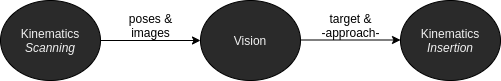
\includegraphics[width=0.5\textwidth]{images/overview}
\end{figure}


To utilize ROS and already existing Franka ROS Library the kinematics package is formed by the following nodes:
\begin{itemize}
    \item simple\_scanner: Employs the scanning routine around the target point to generate image and pose pairs necessary for vision. Holds SphericalScanner class.
    \item simple\_capture: Communicates with scanner node to save necessary information at every stop. Holds ImageCapture class.
    \item simple\_inserter: Manages the insertion procedure given a target point and a peak point. Holds Inserter class.
    \item simple\_planner: Trajectory planner node, plans and publishes the plans on desired control frequency given the goal pose in homogenous transformation. Holds TrajectoryPlanner class.
    \item simple\_goal: A goal definer for debugging purposes. It is created to test the kinematics application not depending on the state of the vision package. Holds GoalSetter class.
\end{itemize}
These active nodes are utilizing the following modules
\begin{itemize}
    \item simple\_node: Holds the Communicative\_Node parent class which is inherited by most of the classes in this package. It maps all the necessary topics while keeping track of whether the process is on simulation. It also has some commonly used methods by most of the other modules such as waiting for execution or getting joint states.
    \item simple\_robot: Holds Robot class that is imported whenever forward kinematics is needed to be employed. It uses the inherent links that are provided by manufacturer and also necessary end effectors which all are broadcasted via tf package from ROS.
    \item simple\_ik: Holds Inverse\_Kinematics class which is executed whenever there is need of inverse kinematics calculation.
    \item simple\_quintics: Includes mostly static mathematical methods that are necessary to plan a trajectory with quintic polynomials.
    \item simple\_cartographer: Helps the trajectory planner when it needs to make end effector point at some point during scanning or insertion processes.
\end{itemize}

A diagram to help visualize the kinematics package can be found in Appendix, Figure \ref{app_overview}.

The entire process can be summarized as
\begin{itemize}
    \item Scanner node starts a spherical scan pattern around the approximate target point whilst directing the camera towards it with the help of Cartographer. During which there is a checkerboard for calibration purposes.
    \item Capture node captures images and poses to pass on Vision package.
    \item Receiving the target point and approach direction Inserter class first peaks at the target point where it can insert the needle on a straight line, then inserts it to the target.
\end{itemize}
During this process Cartographer helps directing the end effector to the desired orientation, Robot class tracks the provided and developped coordinate frames and joint limits, inverse kinematics  calculates the joint states that are needed to be reached for the target point at each step. All of which are passed to the planner which outputs a plan quantized with the control frequency, or in case of insertion fed directly to the command topic of robot.


The entire implementation of this package is done on most recent versions of both Python and ROS, which during the time of the study were 3.9 and Noetic respectively.
Indeed the provided robot framework runs on the Python 2.7 and ROS Kinetic, which has potential to pose a problem via incompatibility.
Although at the end flexible ROS architecture allowed us to run the package on another computer on the same network and communicate controller via topics.
One more implementation note is the use of a modified fork of franka\_ros package.
To be able to communicate the current execution state, franka\_ros package is modified accordingly and stored in a separate fork from the original clone that was provided.


\section{Vision}
In order to navigate and insert the Needle at the target it is important to visualise and understand the properties of it for it to communicate with the corresponding kinematic motion.This is done by capturing images of the target on camera.Thus, it is important to know the properties of the camera, how it is transformed from a 2D to a 3D space and how to align them to the appropriate coordinate frames.

\begin{itemize}
    \item Camera Calibration from which we can get the intrinsic and extrinsic properties of the camera
    \item Hand-Eye Calibration which determines the transformation between the robot's end-effector and the camera frame to bind the 3d information of both the coordinate systems
    \item Model Recording, where we get the information such as shape, size, orientation of the experimental object which in our case is the phantom
    \item Model Registration, where we record the images of the phantom as the robot drives the camera around it and stitches the individual point-clouds to a 3d scan and registers with the target model
\end{itemize}

\subsection{Camera Calibration}
This is the first and fundamental step in order to precisely navigate the robot to the target. A camera has two sets of properties- Intrinsic and Extrinsic. The intrinsic properties describe the distortion, focal length and optical centers of the imaging system while the extrinsic properties include the position and orientation of the camera with respect to the world frame. To calibrate and find the parameters, we use the checkerboard with known properties, since it is easier to detect the corners and patterns which is used to estimate the intrinsic parameters. The camera captures the images of checkerboard from different positions and is thus calibrated accordingly.

\subsubsection{Implementation}~\\
To perform camera calibration of a Kinect Camera 2.0, OpenCV2  and python 2.7 were used. The program coded is similar to the classic calibration examples provided in [7]. In order to get a good result with less re-projection error, about 30-40 images were captured and used for the calibration. Higher the number of samples, lesser the error. We were able to validate our results by comparing it with the manufacturer's provided parameters.

Both RGB and depth images were calibrated and from the results we can extract the intrinsic and extrinsic properties of the camera. The extrinsic property gives the transformation from the camera to checkerboard, which is used in hand eye calibration. Kinect2.0 has two cameras one for infrared and depth and one for RGB.
\begin{equation}
cv.stereoCalibrate()
\end{equation}

In order to prevent misalignment between the two cameras, stereo calibration was also performed where we align the depth and RGB cameras which is reflected from the extrinsic results.

\subsection{Eye-in-Hand Calibration}\label{AA}
Hand-Eye calibration is used to determine the transformation between the robot's end-effector and the camera frame. For many robot assisted medical applications, it is necessary to accurately compute the relation between the robot's coordinate system and the coordinate system of a tracking device (camera in our case). We implemented the method from the paper [5] for getting the hand-eye transformation.
\subsubsection{Setup}~\\
We mounted the camera on the end-effector of the robot and we kept the checkerboard stationary as the the calibration object. On moving the robot to different poses, we captured the images as well as the end-effector's position and orientation at each pose which is used in the method explained below. For a precise hand-eye calibration we require at least 35-40 checkerboard poses which should be taken in good light and at different angles. Thus we took all the poses covered inside the hemispherical trajectory.
\subsubsection{Method}~\\
The paper presented a new variation of simultaneously computing both X and Y using a method called QR24 optimisation. The basic equation that is used to solve the hand eye calibration is
\begin{equation}
AX=YB
\end{equation}
\begin{equation}
T_{gripper}^{base} * T_{camera}^{gripper} = T_{marker}^{base} * T_{camera}^{marker}
\end{equation}
From equation (9) we have the transformation from robot's base to gripper(end-effector) as the camera records the checkerboard and the marker poses from the camera to checkerboard. So with two known and two unknown parameters, we can estimate these matrices using a least squares approach and each matrix X and Y will have 12 estimated elements.
\begin{equation}
X = lstsq(A_{combined}, B_{combined})
\end{equation}Thus we get the hand-eye transformation of end-effector to camera using this method.
Working with the simulation model of the Kinect camera gave precise results compared to the ones taken during the experiment since some poses did not give good calibration. But towards the end we managed to take clear photos of the checkerboard and was able to get the transformation which was comparable with the provided result. This result is in turn used while stitching the point-clouds with the target image to get the position of the target.

\subsection{Model Recording}
Model Recording was a short but important phase of the project. This is done to know the the shape, size and the structure of the experimental object which in our case was the phantom.
\subsubsection{Implementation} ~\\
We used the point cloud data of RGB camera which was calibrated. Point cloud is a set of points in space that gives 3D information of the object by placing the points on the external surface. This point-cloud data is usually recorded in the camera coordinate system,but for making the robot to know where the object is exactly placed in the world, the point cloud is to be transferred to world coordinates. Since we got a great resolution and a perfect image on camera, we proceeded with a single point cloud file for model registration.


\subsection{Point-Cloud Stitching and Model Registration}
As the robot drives the camera, with the help of the robot poses and the result from hand-eye calibration.The recorded point clouds are stitched and combined to one point cloud and this is then registered to a high resolution CAD model obtained from computer tomography.Once its registered the target for the needle is selected in the final step.
\begin{figure}[htbp]
\centerline{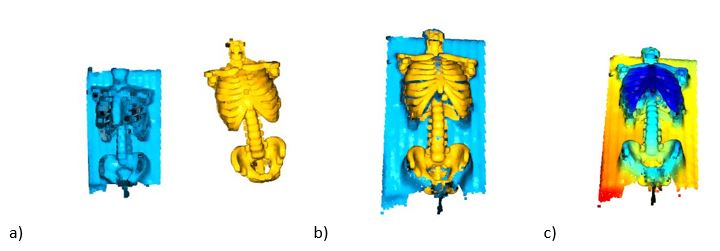
\includegraphics[width =.5\textwidth]{images/finalfig.JPG}}
\caption{a) Initial positions of point-clouds b) Globally registered PointClouds c) Targetpoint selection}
\label{fig}
\end{figure}
\subsubsection{Implementation} ~\\
The phantom was scanned from a single position and we used only one point cloud to perform the registration.
The point-cloud operations were accomplished using Open3D in the version 0.9.0 [6]. It is an open-source library that supports rapid development of software that deals with 3D data.The code was implemented using python 2.7.
The algorithm for performing the model registration and target selection consists of the following steps:
\begin{enumerate}
\item Converting the high resolution CAD model of the phantom to create point-cloud and scale it according to the units used.
\item Stitching and cropping the point cloud so that it only contains the relevant parts
\item Down-sampling the point-clouds and compute Fast Point Feature Histograms(FPFH) features
\item Fast Global Registration using the hand-eye transformation and the obtained pose
\item Local refinement of the registration using point to plane Iterative Closest Point (ICP)
\item Manually choosing the target point from the registered point cloud and transforming it to the world Coordinates.
\end{enumerate}
We used two evaluation metrics, one is the fitness function to measure the overlapping area andthe other is to calculate the RMSE of all inlier correspondences.

\section{Discussion}
\subsection{Kinematics}
Kinematics package overall performs satisfactory to the task at hand. Following remarks can be made on the last state of the implementation:
\begin{itemize}
    \item  Utilizing ROS Service \& Client pairs instead of some of the topics might be more functional although during the study these features were not digested enough by the participants.
    \item  The method of fitting trajectory profiles with quintic polynomials yields smooth movements but it operates mostly on suboptimal range in terms of performance. In this study we took consideration of hardware limits to not to operate with any possible harm to the hardware, so smoothenes of quintics were chosen over performance of other methods. Although other methods can be studied.
    \item Another improvement might be a prelimiary check for target point whether it lays inside the workspace since least squares solution would find the closest point in the workspace even if not reached.
    \item A better inverse kinematics metric separately evaluating orientation and position can be studied.
    \item Instead of evenly sampled points across hypothetical hemisphere during scanning process can be converted to random points to reduce bias, which would be a easy alteration with the numpy.random module.
\end{itemize}    
\subsection{Vision}
To perform the registration we had to decide on the voxel size in order to down sample the point cloud. For voxel sizes between 0-3 we got good results.With fast global registration along with local refinement using ICP we achieved a significant improvement in the fitness function value which was 1.0. The RMSE of the inlier was around 0.0322.This was a pretty good result for model registration.
There were some difficulties in implementing this along with ROS due to version compatibility of Virtual Machine. The Vision on the whole thus, was implemented offline and the target points were obtained and given to the needle insertion package.
\subsection{Contributions}
This report is prepared jointly;
A.K. took the responsibility of Vision section, O.C.T. prepared the rest of the sections and organised the paper, whilst M.D. and K.K. supported with revision and initial templates. Participants explain their parts of the work in the following paragraphs.

\subsubsection{Aishwarya Krishnamurthy} My contributions to the project were to completely implement the Vision package starting from camera calibration up till Point Cloud registration. For model recording  my other teammate Chinmay recorded and collected the point clouds as a rosbag for further processing. The Vision part was completely conducted offline due to version incompatibility of Open3D on my VM. Due to some minor error in the file handling in hand-eye calibration we were not able to get the target from the point cloud, although it worked on the simulation data and the logic and the rest of the code functions well.

\subsubsection{Chinmay Sujir} To get a better understanding of Point Cloud Recording and  Model Registration, ICP and PCL were referred to, along with a Python based PCL named Strawlab library.
While there were no problems in converting and processing  the .PCD files obtained from the ROSBAG using the above mentioned papers and libraries.
Due to the lack of documentation of the Strawlab library and the incompatibility of the converted  ROSBAGS to a .PCD or  .PLY file, for MATLAB ROS toolbox and Vision toolbox. The apporach to Model registration had to be restructured and handed over to  Aishwarya.

\subsubsection{Konika Narendra Khatri } Solving inverse kinematics using Analytical approach involves a lot of matrix algebra and trigonometry.But the advantage of this approach is that once you have drawn the kinematic diagram, derived the equations, computation is fast as compared to Numerical approach. On the other hand the disadvantage is the kinematic diagram and trigonometric equation are exhausting to derive. For each new robotic arm you have to derive new equations, so generalization does not apply over here. I referred Tutorial 5 Geometrical method to solve inverse kinematics using Python and there were some issue in the calculation part of last three joint angles.

\subsubsection{Mansi Dayama} Solved forward kinematics using classic DH formula but then the output was not as expected. So Aishwarya helped in the implementation of forward kinematics using modified DH formula. For trajectory planning, I was working on RRT and RRT* method, did coding for the method  but got some errors and was not sure how to implement this method for Panda robot so did not implement this method. Helped other teammate with research on model registration and trajectroy planning.

\subsubsection{Orhun Cenk Taskin}
Initially part of the vision team, I took over the kinematics part after a reconsideration. When I started kinematics had an initial forward kinematics calculation and an inverse kinematics approach by the initial kinematics team. Then I developped the kinematics package as it is now from scratch with its current architecture and ROS implementation, additionally helping the rest with Python, ROS and managing git repository.

\subsubsection{Sriramkumar Sarida}
My contributions to this project were the implementation of specific tasks alone. I had a separate implementation of Forward and Inverse Kinematics scripts, which are used in the project. Furthermore, I had the initial implementation of the Trajectory planning node using quintic polynomials, which is also used in the project. These programs were coded standalone on python.
\section{Conclusions}
Overall surgical needle insertion with the implementation of modern advancement in computer vision and robotics is an application of surgical robotics that is open for improvement. We employed such techniques to achieve precise needle inseriton, although the vision package wasn't functioning, we were able show functional navigation of the robot. We would like to thank the Institute of Medical Technology and Intelligent Systems for giving us the possibility of working with a real-life surgical robot.

\begin{thebibliography}{1}

    \bibitem{frankaweb}
    Franka Emika,
    \emph{Robot and interface specifications, Franka Control Interface}.
    \href{https://frankaemika.github.io/docs/control_parameters.html}{FCI website}, retrieved in 12.08.2021

    \bibitem{wikidh}
    Wikipedia,
    \emph{Modified DH parameters, Denavit–Hartenberg parameters}.
    \href{https://en.wikipedia.org/wiki/Denavit%E2%80%93Hartenberg_parameters#Modified_DH_parameters}{Wikipedia link}, retrieved in 12.08.2021

    \bibitem{wikikine}
    Wikipedia,
    \emph{Kinematics}.
    \href{https://en.wikipedia.org/wiki/Kinematics}{Wikipedia link}, retrieved in 12.08.2021

    \bibitem{spong}
    Spong, Mark W., Seth Hutchinson, and M. Vidyasagar.
    \emph{Robot modeling and control}. 2006. Hoboken, NJ: John Wiley \& Sons.

    \bibitem{QROptimization}
    Floris Ernst, Lars Richter, Lars Matthaus.
    \emph{Non-orthogonal tool/flange and robot/world calibration}. 2012. International Journal of Medical Robotics Computer Assisted Surgery.

    \bibitem{Open3D}
    \emph{Point-Cloud API Python 0.9.0.0}.
    \href{http://www.open3d.org/docs/0.9.0/tutorial/Basic/index.html}{Link}

    \bibitem{OpenCV}
    \emph{OpenCV CameraCalibration and HandEye calibration}
    \href{https://docs.opencv.org/master/dc/dbb/tutorial_py_calibration.html}{Link}

\end{thebibliography}




\appendix
In this section you can find the appended figures.
\begin{figure*}[ht]
    \centering
    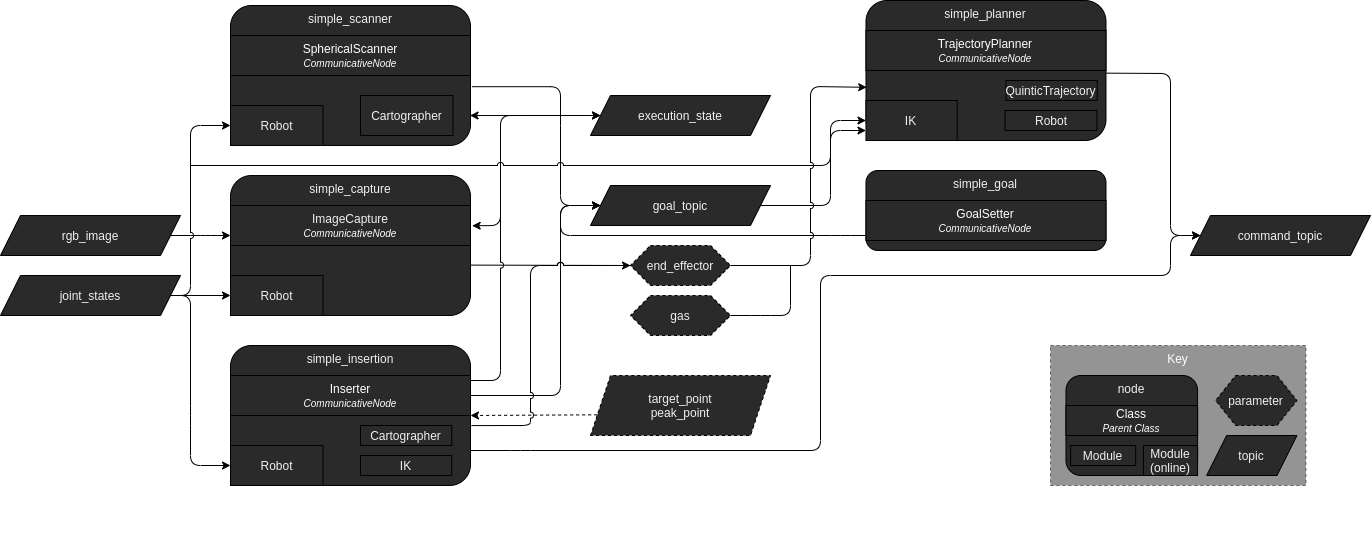
\includegraphics[width=\textwidth]{images/diagram.png}
    \caption{Diagram of the kinematics package}
    \label{app_overview}
\end{figure*}
\newline

\begin{figure*}[ht]
    \centering
    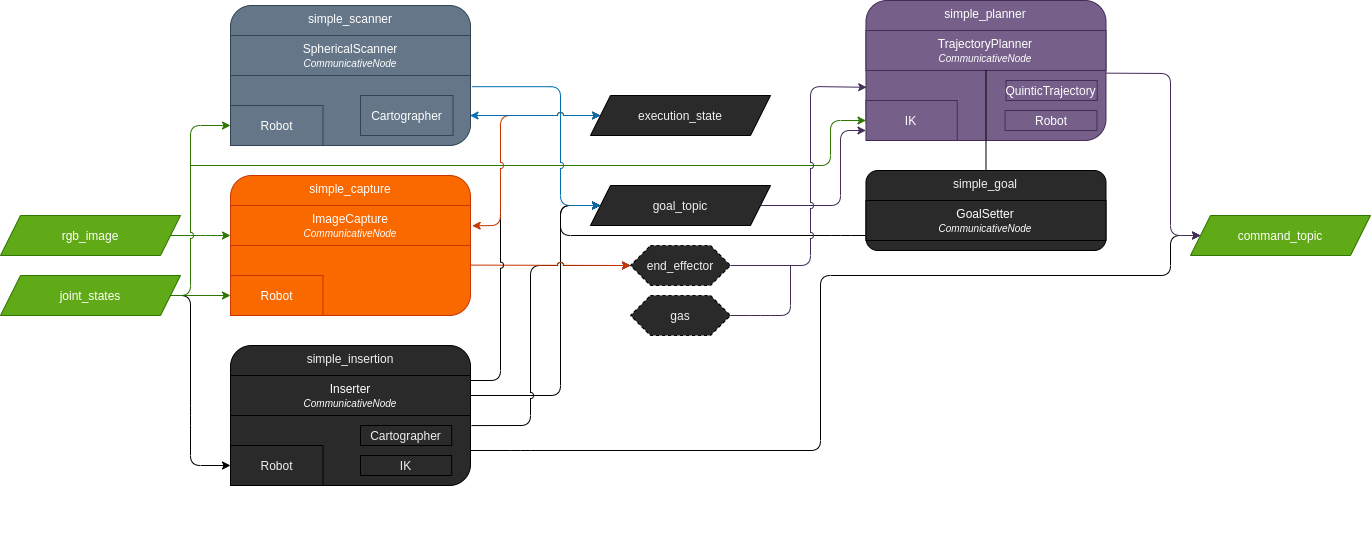
\includegraphics[width=\textwidth]{images/scanning.png}
    \caption{Active nodes during scanning}
    \label{app_2}
\end{figure*}

\newpage


\begin{figure*}[ht]
    \centering
    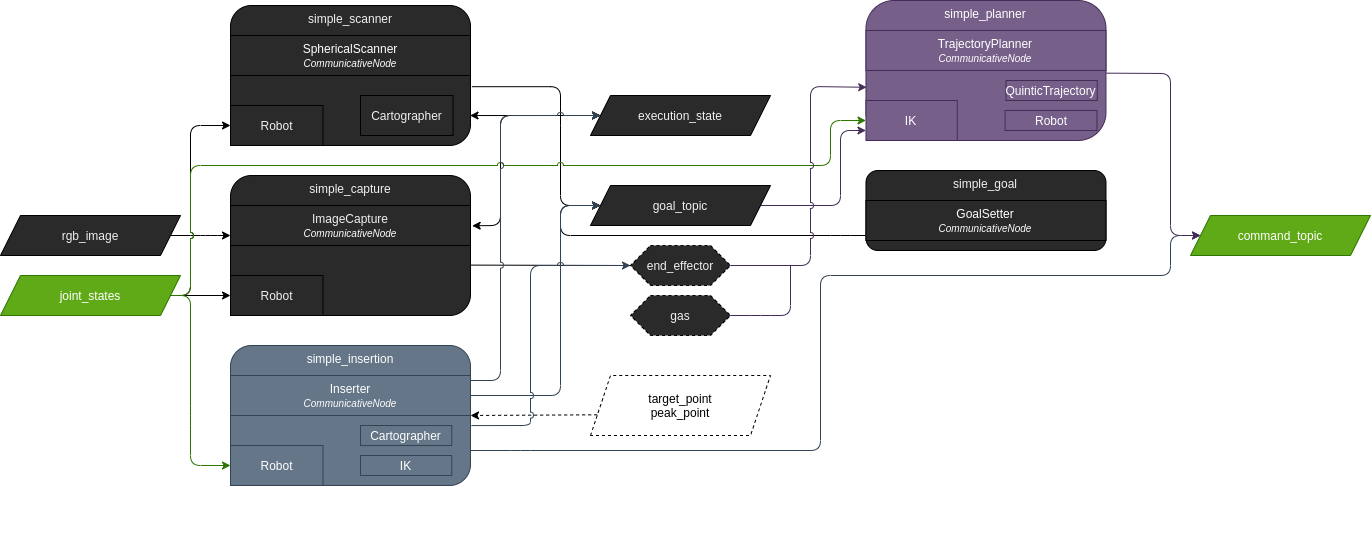
\includegraphics[width=\textwidth]{images/insertion.png}
    \caption{Active nodes during insertion}
    \label{app_3}
\end{figure*}

\end{document}
